% English master manuscript. Target: exactly six pages including references.
\documentclass[conference]{IEEEtran}
\IEEEoverridecommandlockouts
\usepackage{fontspec}
\setmainfont{Times New Roman}
\setsansfont{Arial}
\setmonofont{DejaVu Sans Mono}
\usepackage{graphicx}
\graphicspath{{figures/}}
\usepackage{amsmath,amssymb}
\usepackage{booktabs}
\usepackage{array}
\usepackage{url}
\usepackage{balance}
\usepackage{microtype}

\title{Radar-Only, Camera-Gated, and Emergency-Fallback AEB: Scenario-Level Trade-offs and Failure Severity in CARLA}

\author{
\IEEEauthorblockN{Mai Viet Hoang and Duc An Pham}
\IEEEauthorblockA{\textit{Hanoi University of Science and Technology}\\
Hanoi, Vietnam\\hoangmai04222@gmail.com}
}

\begin{document}
\maketitle

\begin{abstract}
Camera permission gating can suppress radar-triggered false braking but veto
hazards outside a detector's label space. We compare radar-only, hard camera
gating, and camera gating with a conservative radar emergency fallback in a
sensor-to-brake automatic emergency braking (AEB) pipeline in CARLA 0.9.11.
Unlike a run-count analysis, the primary unit is a named condition: 105 core
conditions and a 14-condition frozen adverse hold-out, each repeated five times
only to check consistency. On core, radar-only, hard-gate, and fallback policies
respectively obtain scenario-level precision/recall of 0.913/0.988,
1.000/0.965, and 1.000/0.988; fallback passes 101/105 conditions. This does not
generalize as dominance. Hard gating passes 11/14 hold-out conditions versus
7/14 for fallback because four convincing synthetic-ghost conditions pass the
fallback rules. Those fallback false brakes are severe in simulation: all 20
repeated runs stop from a median 78.4~km/h, with 3.60-s braking and
9.02~m/s$^2$ median peak deceleration. Physical-prop collisions further show
why brake recall is insufficient: on an unseen bench, radar-only reduces the
last pre-impact speed to 32.57~km/h, while delayed fallback reaches
54.93~km/h and hard gating 59.95~km/h. A frozen 2,461-run CUDA campaign,
component ablation, perturbations, detector disabling, explicit scoring, and
traceable logs support an empirical map of precision--recall and failure
severity---not a general fusion advantage or safety certification.
\end{abstract}

\begin{IEEEkeywords}
automatic emergency braking, radar--camera gating, CARLA, false braking,
precision--recall, fault injection, scenario-level evaluation
\end{IEEEkeywords}

\section{Introduction}
AEB closes a perception--decision--actuation loop in which a sensor detection
must become a timely and justified brake. Radar supplies range and radial
velocity but can select non-hazards or spurious returns. Camera semantics can
reject implausible radar targets, yet a missed or out-of-label object is not
proof of free road. Reviews therefore treat sensing, target selection, risk,
and control as an interdependent chain \cite{yang2022aebreview}.

Radar--vision AEB recognition and noise filtering are established
\cite{kim2013vehicle,hsu2015noise}. A recent preprint specifically studies
radar-guided camera verification \cite{akula2026radarguided}. This paper does
not claim a new fusion primitive. It asks a narrower empirical question: can a
late radar emergency override recover non-vehicle hazards rejected by a
car-only camera gate without restoring radar false brakes, and which failure
mechanisms prevent that goal?

Simulation enables repeatable near-collision tests
\cite{dosovitskiy2017carla,kang2019testing}, but two practices can overstate
evidence: using privileged actor truth online, and treating deterministic
repetitions as independent samples. We use only CARLA radar points and RGB
frames for braking, reserve actor truth for offline labels, freeze policy and
suite before hold-out, and make named conditions the primary unit. Repetitions
measure process consistency. We also augment binary brake/collision counts with
false-brake duration/deceleration and last-tick pre-impact speed.

The contributions are: (1) a paired comparison of radar-only, hard gate, and
emergency fallback; (2) scenario-level confusion, Wilson descriptors, and
paired system outcomes; (3) ablation, one-factor sensitivity, local
perturbation, detector-disabled, and frozen adverse hold-out tests; and (4) a
2,461-run resumable GPU protocol with provider, hash, tick, and failure-severity
traceability. The central result is both positive and negative: fallback
combines the two core operating points, while high-support ghosts and late or
missing physical tracks preclude a dominance claim.

\section{Related Work and Positioning}
Kim and Song combine radar and vision for AEB vehicle recognition
\cite{kim2013vehicle}; Hsu \emph{et al.} filter radar/camera noise for target
selection \cite{hsu2015noise}. Bae \emph{et al.} estimate the closest in-path
vehicle through LiDAR projection and camera tracking on a real vehicle
\cite{bae2021cipv}; Zhang \emph{et al.} combine curved-road target selection,
TTC, safety distance, and graded braking \cite{zhang2023curved}. CenterFusion
illustrates learned radar--camera association for 3-D detection
\cite{nabati2021centerfusion}, whereas our policies keep radar kinematics and
camera permission explicitly separable for controlled substitution.

CARLA supports protocol-derived pipeline evaluation
\cite{gomez2022carla}; recent CARLA AEB work also evaluates alternative visual
sensing \cite{feng2025dvs}. Virtual radar fidelity depends strongly on whether
the model represents objects, detections, or raw signals
\cite{magosi2022radar}. Our contribution is therefore a falsification-oriented
late-policy comparison, not a claim that point-level CARLA radar reproduces
multipath prevalence. Standards motivate scenario structure but are not
reproduced as compliance tests \cite{iso15623,euroncap_aeb}.

Two distinctions position the present study. First, object-level learned fusion
usually seeks detection accuracy, while an AEB permission gate asks whether an
already collision-relevant radar track may actuate. A missed camera association
therefore has asymmetric cost: it may prevent a false brake or veto a genuine
hazard. Second, simulation papers often report nominal success without an
adverse set frozen before evaluation. Here the same attributes used to justify
fallback---persistence, centrality, support, and critical risk---are deliberately
reproduced by a synthetic fault after policy freeze. The contribution is the
resulting policy/failure comparison and audit trail, rather than a new detector,
tracker, or standards procedure.

\section{System and Policies}
\subsection{Information boundary and configuration}
The ego Tesla Model 3 runs on Town04 in synchronous 0.05-s steps. Table~\ref{tab:setup}
reports the frozen sensor and detector settings. Camera and radar both tick at
0.05~s; YOLO inference is scheduled by simulation timestamp at 0.15~s, and
confirmation is held for 0.35~s. Online code does not query actor identity,
class truth, target velocity, or ground-truth boxes.

\begin{table}[t]
\caption{Frozen sensing and detector setup.}
\label{tab:setup}
\centering\scriptsize
\setlength{\tabcolsep}{3pt}
\begin{tabular}{p{0.28\columnwidth}p{0.65\columnwidth}}
\toprule Item & Setting\\ \midrule
Camera & RGB, 1280$\times$720, $70^\circ$ FOV; $(x,z)=(0.43,1.35)$ m\\
Radar & 100 m, $30^\circ\!\times6^\circ$, 2000 points/s; $(x,z)=(2.53,0.48)$ m\\
Detector & YOLO26n ONNX \cite{ultralytics_yolo}, 640 input, confidence 0.25, NMS IoU 0.50\\
Dataset & 1505/300/200 train/val/test images; 28/6/4 disjoint collection sessions\\
Training & one \emph{car} class, AdamW, seed 2026; ONNX SHA-256 prefix \texttt{dc0a6ca1754a}\\
Runtime & CUDA required, 0.15-s inference cadence, 0.35-s confirmation hold\\
\bottomrule
\end{tabular}
\end{table}

Dataset splits contain 1872/379/264 instances, no exact cross-split image
duplicates, and 21.2/16.3/18.0\% empty frames. Split session identifiers are
disjoint, rather than interleaving adjacent frames across splits, although all
imagery remains Town04 in-domain. Validation precision, recall,
$\mathrm{mAP}_{50}$, and $\mathrm{mAP}_{50:95}$ are 0.9919, 0.9642, 0.9940,
and 0.9495; these do not establish out-of-domain safety. Exact radar-to-camera
transforms project a selected target into the current image. A confirmation
requires its projected point inside a retained car box after confidence and NMS
filtering. Sensor callbacks carry simulation-frame timestamps; inference cadence
and hold expiry use simulation rather than host time. The 0.35-s hold intentionally
bridges the 0.15-s inference cadence, but also defines a bounded stale-semantic
window that is identical for both camera policies.

Radar points are filtered by range, road height, and a predicted
constant-curvature path, clustered by position/velocity, and associated across
frames. A target track must be confirmed, non-stale, and collision-relevant.
For distance $d$, relative radar velocity $v_r<0$, and ego speed $v_e$,
\begin{equation}
 v_c=-v_r,\quad \mathrm{TTC}=d/v_c,\quad v_t=\max(0,v_e+v_r).
\end{equation}
The stopping requirement and margin are
\begin{equation}
 d_{\rm req}=\max\!\left(d_0,v_et_r+\frac{v_e^2}{2a_e}-
 \frac{v_t^2}{2a_t}+d_0\right),\quad m=d-d_{\rm req},
\end{equation}
with $t_r=0.20$~s, $a_e=8$, $a_t=6$~m/s$^2$, and $d_0=1$~m as simulation
risk parameters. A staged PID maps risk to continuous CARLA brake.

\subsection{Three late brake policies}
Radar-only passes the radar AEB decision $B_r$. Hard gating requires current
camera confirmation $C$ or held confirmation $H$. The emergency policy is
\begin{equation}
 B_f=B_r\land(C\lor H\lor E_r).
\end{equation}
$E_r$ requires a confirmed/non-stale track, age and hit streak $\geq3$, at
least six cluster points, confidence $\geq0.70$, absolute path offset
$\leq0.65$~m, TTC $\leq1.10$~s, and margin $m\leq-2.0$~m. TTC and margin are
conjunctive. Once accepted, fallback latches until radar exits \texttt{BRAKE}.
A camera box cannot create kinematic risk without a radar target. Thus all
policies share radar processing, equations, PID, scenario control, and scoring;
only brake permission differs.

The fixed online order is: update ego path; filter points; update and confirm
tracks; select one radar target; evaluate TTC/margin; process the latest camera
frame when cadence permits; apply the selected permission policy; command the
staged PID; and log the following simulator state. This boundary prevents a
camera box from inventing range or relative velocity and prevents actor truth
from repairing a weak radar track. It also localizes policy differences: a
missing cluster fails before every gate, while a confirmed but unlabelled track
separates hard gate from fallback.

\section{Frozen Protocol and Outcome Definition}
The v1 thresholds, named suites, and protocol were repository-tagged before
hold-out execution. Hard gate and fallback use the same ONNX model and required
\texttt{CUDAExecutionProvider}; provider fallback or inference error is a
technical hard stop. All repetitions of one named condition execute in a fresh
CARLA process before the next server. Algorithmic failures are retained.

The campaign contains 2,461 runs in 639 process-isolated sessions. Core has a
66-condition CCRm/CCRb/cut-in speed--gap sweep, 29 mixed vehicle/negative
regressions, eight lateral edge props, and two central box/barrel hazards. Six
weak four-point synthetic-fault conditions are analysed separately. Local
robustness adds 20 speed ($\pm2$~km/h), gap ($\pm1$~m), cut-in-time
($\pm0.1$~s), and prop-offset ($\pm0.15$~m) perturbations. Ten detector-disabled
conditions test complete loss of camera detections. The frozen adverse hold-out
contains three new central prop types, four vehicle appearances, two new edge
props, and five persistent ghost geometries with 6--10 injected points.

Core and hold-out conditions are repeated five times; development and
perturbation use two and three repeats. The fixed seed is recorded as 2026.
Every reported named cell is consistently all-PASS or all-FAIL over its repeats;
thus the named condition---not the run---is the primary descriptive unit. The
large run total documents execution coverage, restart behavior, and repeatability
but is not presented as 2,461 independent traffic encounters.

Labels are assigned in frozen YAML before execution. A positive prediction
means at least one tick with \texttt{aeb\_override=true}. Collision means any
tick with \texttt{collision\_count>0}. System PASS requires brake/no-brake and
collision to equal their expectations; positive non-collision cases also
require minimum bumper gap $\geq0.5$~m, while selected scenarios enforce frozen
lane/target assertions. Hence a brake TP may still collide and fail.

We report named-condition TP/FP/TN/FN, PASS, collision, and paired status.
Wilson intervals use named-condition counts only and remain finite-grid
descriptors, not road-population inference. Suite class ratios are designed.
Severity is derived without rerunning CARLA: pre-impact speed is the last
0.05-s tick before first collision; false-brake duration counts override ticks;
peak deceleration excludes initialization, sub-1-km/h, and collision ticks.
This discrete pre-impact proxy can differ from contact-point speed within one
simulation tick and is reported as such. Paired PASS matrices use identical
condition identifiers. No null-hypothesis significance test is used because the
grids are deliberately constructed rather than randomly sampled from a traffic
population.

\section{Results}
\subsection{Scenario-level core and hold-out trade-off}
Table~\ref{tab:primary} and Fig.~\ref{fig:primary} replace run-level uncertainty
with named-condition analysis. On core, fallback passes 101/105, versus 99 for
hard gate and 93 for radar-only. It restores two non-vehicle conditions missed
by hard gating and rejects eight edge-prop conditions that trigger radar-only.
The eight radar-only false-positive conditions are four prop types at two
lateral offsets; hard gate and fallback reject all. Conversely, radar and
fallback brake for both central box/barrel conditions, while the car-only hard
gate produces two FN/collisions. All policies also share one FN at a late
lateral-corridor cut-out boundary. The three shared collision conditions are two
high-speed braking-lead cases and one shortest high-speed cut-in. Hard gate adds
the two central-prop collision/FN conditions. Across five consistency repeats this corresponds to 15/25/15
collisions, but those run totals are not independent sample sizes.

\begin{table*}[t]
\caption{Primary named-condition results; intervals are 95\% Wilson descriptors over the constructed condition grid.}
\label{tab:primary}
\centering\scriptsize
\setlength{\tabcolsep}{3pt}
\begin{tabular}{llrrrrrccrr}
\toprule Scope & Policy & N & TP & FP & TN & FN & Precision [CI] & Recall [CI] & PASS & Coll.\\
\midrule
Core & Radar & 105 & 84 & 8 & 12 & 1 & .913 [.838,.955] & .988 [.936,.998] & 93 & 3\\
 & Hard & 105 & 82 & 0 & 20 & 3 & 1.000 [.955,1] & .965 [.901,.988] & 99 & 5\\
 & Fallback & 105 & 84 & 0 & 20 & 1 & 1.000 [.956,1] & .988 [.936,.998] & 101 & 3\\
\midrule
Hold-out & Radar & 14 & 6 & 5 & 2 & 1 & .545 [.280,.787] & .857 [.487,.974] & 6 & 3\\
 & Hard & 14 & 5 & 0 & 7 & 2 & 1.000 [.566,1] & .714 [.359,.918] & 11 & 3\\
 & Fallback & 14 & 6 & 4 & 3 & 1 & .600 [.313,.832] & .857 [.487,.974] & 7 & 3\\
\bottomrule
\end{tabular}
\end{table*}

Six additional weak four-point synthetic-fault conditions are excluded from
primary core confusion: radar-only falsely brakes in all six, while both camera
policies block all. Including them would lower radar precision but leave the two
camera-policy estimates unchanged; exclusion keeps the primary table focused on
physical actors/props and ordinary negative scenarios. In paired core system
status, fallback versus hard gate has 99 both-PASS, two fallback-only PASS, zero
hard-only PASS, and four both-FAIL conditions. The scenario-level Wilson bounds
are visibly wider than the former run-level bounds; for example hard-gate core
precision has lower bound 0.955 rather than 0.991. This is the intended
statistical correction, not evidence that the point estimate changed.

\begin{figure*}[t]
\centering
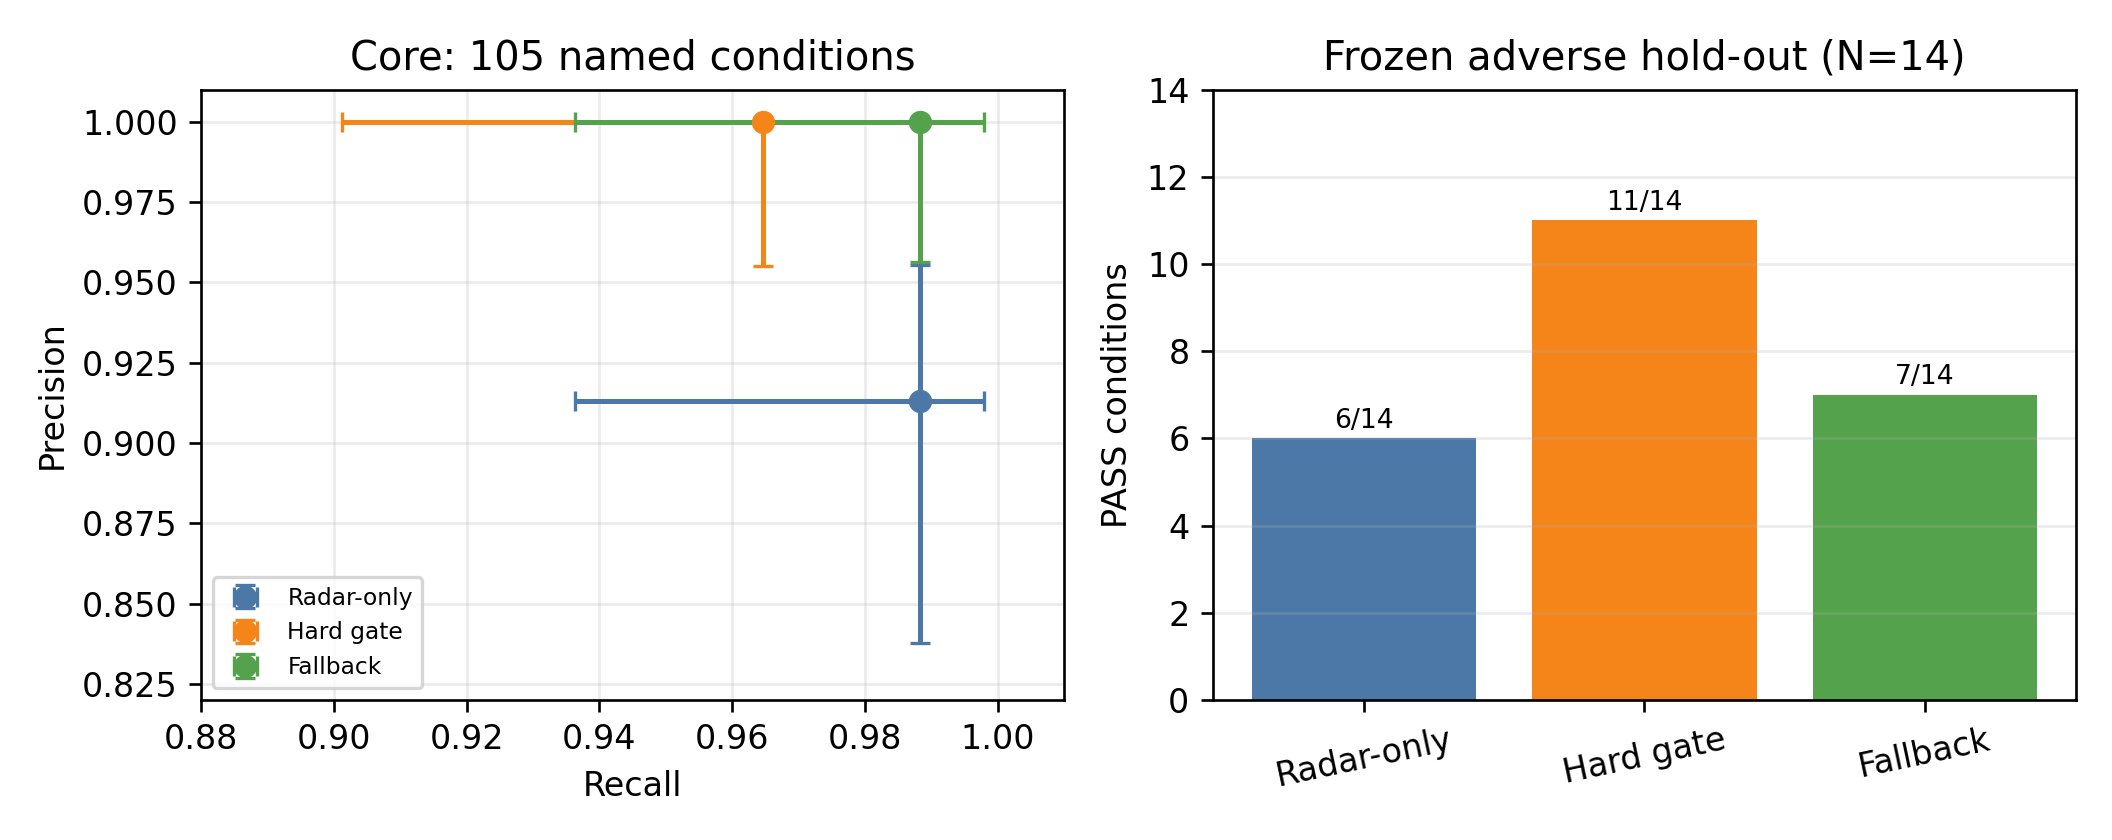
\includegraphics[width=0.92\textwidth]{scenario_level_tradeoff.png}
\caption{Named-condition evidence. Left: core precision--recall with descriptive
Wilson intervals. Right: system PASS on the 14-condition frozen adverse
hold-out. Neither grid represents road prevalence.}
\label{fig:primary}
\end{figure*}

Hold-out reverses the apparent dominance. It contains three unseen central
props, four vehicle appearances, two edge props, and five persistent 6--10-point
synthetic ghosts. Hard gate alone passes four high-support ghost conditions;
fallback alone passes none; both pass seven and both fail three. Fallback blocks
only the 0.75-m-offset ghost. The ghost returns intentionally reproduce the
fallback's rule-level attributes, so this is a mechanism falsification test, not
an estimate of real radar multipath frequency. The label and injection geometry
are fixed in YAML: a closing virtual cluster persists near the predicted center
path while point count and offset cross the frozen fallback boundaries. Calling
this set an ``adverse mechanism hold-out'' avoids implying an independently
sampled deployment distribution.

Vehicle-appearance conditions do not separate hard gate and fallback; the
camera label space still covers them. Physical props and ghosts do. This
mechanism-level decomposition is more informative than aggregate F1: fallback
adds brake recall for unlabelled tracks, but a track-quality rule has no
independent evidence of physical existence.

\subsection{Mechanism decomposition}
The three physical prop failures occur at different pipeline boundaries. The
shopping cart produces at most two path candidates but no confirmed cluster;
therefore radar risk never requests a brake and no late permission policy can
recover it. This is a radar formation/representation failure, not evidence that
the camera veto alone caused impact. The bench does form a confirmed track.
Radar-only responds first, fallback waits for simultaneous point, path, TTC, and
margin qualification, and hard gating receives no usable car confirmation. The
traffic-warning prop is different again: all policies brake at the same gap,
and camera-policy logs show confirmation rather than fallback. Despite early
permission, configured vehicle/prop contact dynamics still produce collision.
The three categories are consequently missing track, late emergency
qualification, and collision despite permission.

Ghosts isolate the opposite path through the system. A six-point center
injection forms one confirmed track by 0.15~s with confidence 1.0,
TTC 0.89~s, and margin $-15.21$~m; radar-only and fallback immediately request
emergency brake, whereas hard gate has no car confirmation. Eight- and ten-point
center/0.50-m ghosts behave similarly. Moving the injection to 0.75~m leaves
radar-only unchanged but crosses the fallback's frozen 0.65-m path threshold.
Thus the adverse outcome follows directly from the stated rule rather than an
unobserved YOLO timing anomaly.

The regression FN is also kept separate. In five repeats of a late cut-out, the
radar target leaves/re-enters the predicted lateral corridor around the decision
boundary and no policy brakes. Pooling that condition, high-speed stopping-limit
collisions, unknown props, and ghosts into one failure rate would hide which
stage can plausibly be improved.

\subsection{Ablation, sensitivity, and controlled degradation}
A 12-condition development ablation, repeated twice, gives full fallback 12/12.
Hard gate and no-latch each fail two central box/barrel conditions. Removing the
central-path constraint creates three edge-prop false-brake conditions; removing
minimum point count creates two weak-ghost false-brake conditions. Removing
stability/confidence or replacing TTC-AND-margin by OR changes none of this
focused grid, so independent necessity is not claimed. In six one-factor
conditions, lowering point count creates one false brake; increasing stability
or tightening TTC each misses one central prop. Other local variants do not
change outcomes.

\begin{table}[t]
\caption{Extended named-condition outcomes.}
\label{tab:extended}
\centering\scriptsize
\setlength{\tabcolsep}{3pt}
\begin{tabular}{llrrrrrrr}
\toprule Suite & Policy & Pass/N & TP & FP & TN & FN & Coll.\\ \midrule
Perturb. & Radar & 19/20 & 20 & 0 & 0 & 0 & 1\\
 & Hard & 15/20 & 15 & 0 & 0 & 5 & 5\\
 & Fallback & 18/20 & 20 & 0 & 0 & 0 & 1\\
\midrule
Camera off & Hard & 4/10 & 0 & 0 & 4 & 6 & 6\\
 & Fallback & 8/10 & 6 & 0 & 4 & 0 & 2\\
\bottomrule
\end{tabular}
\end{table}

In perturbation, fallback's 19-m box collides; its 21-m box avoids collision but
stops at 0.353~m, below the frozen 0.5-m criterion. This corrects the ambiguity
that would result from equating all system FAILs with collisions. With camera
disabled, fallback brakes on all six positive conditions but collides in two;
brake recall again does not imply safe stopping. Hard gating's 4/10 camera-off
PASS conditions are all true negatives, so its apparent system rate should not
be interpreted as hazard capability.

These grids are one-factor local probes, not global threshold optimization.
Specifically, unchanged outcomes for confidence, margin, path, or permissive TTC
variants mean only that the selected six conditions did not cross those
boundaries. They do not prove the rule is unnecessary. Conversely, the point,
path, and latch ablations deliberately contain mechanisms expected to expose
them; effect magnitude is therefore suite-dependent.

\subsection{Failure severity and computation}
Table~\ref{tab:severity} separates three physical mechanisms. The cart yields no
confirmed radar cluster, so all policies impact without braking at 49.96~km/h.
The bench yields a track: radar-only brakes at 12.62~m and reaches 32.57~km/h at
the last pre-impact tick; fallback waits until 4.29~m and reaches 54.93~km/h;
hard gate never brakes and reaches 59.95~km/h. For the warning prop, all policies
brake at 21.87~m---including apparent camera confirmation---and reach
7.82~km/h, so a binary collision count hides substantial mitigation.

\begin{table}[t]
\caption{Frozen hold-out failure severity (median over five consistent runs).}
\label{tab:severity}
\centering\scriptsize
\setlength{\tabcolsep}{3pt}
\begin{tabular}{llrr}
\toprule Mechanism & Policy & Onset / gap & Severity outcome\\ \midrule
Cart & All & no brake & 49.96 km/h pre-impact\\
Bench & Radar & 12.62 m & 32.57 km/h pre-impact\\
 & Hard & no brake & 59.95 km/h pre-impact\\
 & Fallback & 4.29 m & 54.93 km/h pre-impact\\
Warning & All & 21.87 m & 7.82 km/h pre-impact\\
\midrule
Ghost FP & Radar (25 runs) & 78.4 km/h & 3.60 s / 9.02 m/s$^2$\\
 & Fallback (20) & 78.4 km/h & 3.60 s / 9.02 m/s$^2$\\
\bottomrule
\end{tabular}
\end{table}

Every ghost FP is a full simulated stop below 1~km/h, not a one-tick pulse; the
last column reports brake duration/peak deceleration for those rows. This makes
the binary precision loss operationally meaningful inside simulation, although
no following vehicle or occupant model converts it to crash risk. Conversely,
core system-limit collisions occur at approximately 20.43, 37.34, and
77.81~km/h pre-impact under all policies, locating them downstream of the gate.
The bench result adds another nuance: radar-only still fails binary system PASS,
but its 27.4-km/h reduction relative to hard gate represents substantial impact
mitigation that collision count alone would erase. Fallback brakes later and
reduces only 5.0~km/h relative to hard gate.

Across 474 required-CUDA sessions, 74,928 inferences complete with zero errors.
Session-median p50/p95 are 9.95/11.53~ms; weighted mean is 11.56~ms. Each fresh
process has one $>150$-ms cold start; maximum is 276.10~ms. These are ONNX host
processing times under synchronous simulation, not end-to-end ECU deadlines.
They exclude radar preprocessing, callback transport, control application,
display, and vehicle actuation. The one-per-process cold event is retained rather
than discarded as an outlier, because process isolation is part of the protocol.

\subsection{Traceability and audit}
Each child summary records scenario/run identifiers, expected and actual brake,
collision, minimum gap, first brake time/speed/gap, target association, fallback
reason, and failure text. Tick CSV adds point, cluster, confidence, TTC, margin,
command, provider, and collision state. Session manifests record commit, seed,
CARLA client/server version, model/config SHA-256, configured/active execution
provider, inference counts, errors, and latency quantiles. Checkpoint keys are
$(\mathrm{scenario\ id},\mathrm{run\ index})$, so a technical retry replaces an
incomplete run rather than duplicating evidence. The checked derivation script
regenerates named confusion, paired outcomes, collision severity, and
false-brake severity from the frozen raw archive without changing a run.

\section{Discussion and Validity Boundaries}
\subsection{Design implications}
The policies encode different error costs. Hard gating is conservative when a
car-only detector covers the hazard, but structurally rejects unlabelled
objects. Fallback restores selected radar recall while accepting stable,
central, high-support ghosts. Track age, point count, confidence, path offset,
TTC, and margin are attributes of one radar estimate; none independently proves
physical existence. Threshold tuning therefore moves the operating point and
can delay genuine braking, as the bench, sensitivity, and camera-off results
show. New evidence---free space, broader semantics, occupancy, calibrated
existence probability, or richer radar cues---is needed to break that symmetry.

Policy choice should therefore follow explicit error cost. Where unnecessary
high-deceleration braking is dominant, hard gating is favored on this grid; where
camera availability or non-vehicle recall dominates, fallback provides partial
recovery but requires a stronger existence model. Radar-only remains a useful
upper envelope for what the shared radar risk stage can request, not a road-ready
policy conclusion. Failure severity should accompany confusion: the warning
case shows collision mitigation despite system FAIL, whereas ghost cases show
that a false positive can be a complete emergency stop.

\subsection{Validity boundaries}
The study's strength is controlled substitution and adverse evidence, not broad
algorithmic novelty. It does not compare learned or probabilistic fusion,
confidence-matched soft gates, or multi-class/free-space perception. External
validity is limited by one map/ego, one fixed seed, favorable imaging, an
in-domain session-separated dataset, point-level CARLA radar, and deterministic
repeats. Synthetic ghosts are deliberately constructed, not measured
multipath distributions. The adverse hold-out has only 14 designed conditions;
its wide intervals make that limitation visible. No weather/friction sweep,
hardware-in-the-loop, actuator/communication delay, real radar/camera data, or
vehicle test is included. False-brake duration/deceleration and last-tick
pre-impact speed improve binary reporting but are not occupant-risk or jerk-cost
models. The scenarios do not certify ISO or Euro NCAP compliance.

All child runs store commit, seed, model/config SHA-256, CARLA versions, active
provider, and tick-level gate reasons. Raw CSV/JSON, snapshots, manifests, the
derivation script, and archive SHA-256 reproduce both run- and scenario-level
results. This supports auditability, not road-population inference.

A stronger next protocol should pre-register a stochastic fault surface rather
than one threshold-directed ghost: point support 4--12, lateral offset
0--1~m, persistence, range-rate noise, and intermittent returns across multiple
seeds. It should add at least one map, weather/illumination change, friction
levels, and a second ego platform. Competing policies should include a
confidence-matched soft gate, multi-class/free-space visual evidence, and a
probabilistic existence tracker. Evaluation should retain named-condition
pairing while adding impact speed, brake duration, jerk-aware false-brake cost,
and time-to-last-safe-brake objectives. Recorded or hardware-in-the-loop radar
would then test whether the mechanism map transfers beyond CARLA abstractions.

\section{Conclusion}
On a constructed core grid, emergency fallback combines hard-gate precision and
radar-only recall. On a frozen adverse hold-out, hard gating passes more
conditions because fallback accepts convincing synthetic ghosts, while all
policies retain distinct missing/late-track physical failures. Scenario-level
statistics and severity reveal information hidden by repeated run totals and
binary collision counts. Camera gating is therefore false-positive suppression
and radar emergency fallback a conditional trade-off---neither is a general
safety solution.

\balance
\bibliographystyle{IEEEtran}
\bibliography{references}
\end{document}
